\documentclass[aspectratio=169,11pt]{beamer}

\usetheme{default}
\usecolortheme{dove}
\setbeamertemplate{navigation symbols}{}
\setbeamertemplate{footline}[frame number]
\setbeamertemplate{frametitle}{\vspace{0.3cm}\insertframetitle}

\usepackage[T1]{fontenc}
% \usepackage{lmodern}
\usepackage{amsmath,amssymb}
\usepackage{mathtools}
\usepackage{tikz}
\usetikzlibrary{positioning,arrows.meta,calc,fit,decorations.pathreplacing,backgrounds}
\usepackage[table]{xcolor}
\usepackage{array}
\usepackage{booktabs}

\pdfstringdefDisableCommands{\def\translate#1{#1}}

\renewcommand{\leq}{\leqslant}
\renewcommand{\geq}{\geqslant}
\newcommand{\Oh}{\mathcal{O}}
\newcommand{\strips}{\mathtt{strips}}

\definecolor{nczone}{RGB}{168,184,230}
\definecolor{darkblue}{RGB}{40,60,120}
\definecolor{darkred}{RGB}{150,30,30}
\definecolor{slab1}{RGB}{230,180,180}
\definecolor{slab2}{RGB}{180,200,230}
\definecolor{slab3}{RGB}{200,230,180}
\definecolor{slab4}{RGB}{245,225,160}
\definecolor{slab5}{RGB}{210,195,230}
\definecolor{updatezero}{RGB}{176,52,54}
\definecolor{updateone}{RGB}{48,140,97}
\definecolor{splitpiece}{RGB}{118,188,228}
\definecolor{coarsefill}{RGB}{202,211,225}
\definecolor{softgreen}{RGB}{226,242,232}
\definecolor{softred}{RGB}{248,228,228}

\setbeamercolor{block title}{bg=darkblue!15,fg=darkblue}
\setbeamercolor{block body}{bg=darkblue!5}
\setbeamercolor{block title alerted}{bg=darkred!15,fg=darkred}
\setbeamercolor{block body alerted}{bg=darkred!5}

\newcommand{\fillslab}[6]{\fill[#1,opacity=0.66] ({#4-1},{#6-#3}) rectangle ({#5},{#6+1-#2});}
\newcommand{\drawslab}[6]{\draw[#1,very thick] ({#4-1},{#6-#3}) rectangle ({#5},{#6+1-#2});}

\title{Dynamic data structures for twin-ordered matrices}
\subtitle{Queries and updates in \texorpdfstring{$\Oh(\log\log n)$}{O(log log n)} expected worst-case time}
\author{B.~Bosek \and J.~Czy\.{z}ewska \and E.~Kipouridis \and W.~Nadara \and M.~Pilipczuk \and K.~W\k{e}grzycki \and A.~Zych-Pawlewicz}
\institute{Jagiellonian University \quad University of Warsaw \quad MPI for Informatics}
\date{LATIN 2026}

\begin{document}

%% ============== SLIDE 1: Title ==============
\begin{frame}
\titlepage
\end{frame}

%% ============== SLIDE 2: Object ==============
\begin{frame}{What is the dynamic object?}
\begin{columns}[T]
\begin{column}{0.52\textwidth}
\vspace{0.15cm}
{\Large $M \in \{0,1\}^{n\times n}$}
\smallskip
\begin{itemize}
\setlength\itemsep{0.25em}
\item Rows and columns stay in a fixed order
\item After every flip, $M$ is promised to be $d$-twin-ordered
\item We need online cell queries and single-cell flips
\end{itemize}
\smallskip
\begin{beamercolorbox}[wd=\linewidth,sep=0.75ex,rounded=true]{block body alerted}
\footnotesize The challenge is to keep a compact representation without rebuilding it from scratch after each update.
\end{beamercolorbox}
\smallskip
{\scriptsize\color{gray} The fixed order is part of the input; we are not allowed to reorder after updates.}
\end{column}
\begin{column}{0.44\textwidth}
\centering
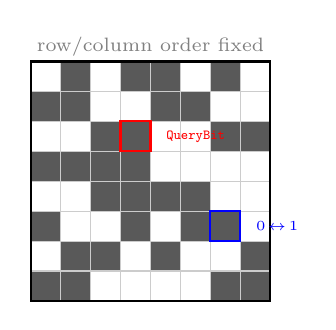
\begin{tikzpicture}[scale=0.38]
\foreach \r/\data [count=\ri from 0] in {
  0/{0,1,0,1,1,0,1,0},
  1/{1,1,0,0,1,1,0,0},
  2/{0,0,1,1,0,0,1,1},
  3/{1,1,1,1,0,0,0,0},
  4/{0,0,1,1,1,1,0,0},
  5/{1,0,0,1,0,1,1,0},
  6/{0,1,1,0,1,0,0,1},
  7/{1,1,0,0,0,0,1,1}}{
  \foreach \v [count=\ci from 0] in \data {
    \ifnum\v=1 \fill[black!65] (\ci,7-\ri) rectangle ++(1,1);
    \else \fill[white] (\ci,7-\ri) rectangle ++(1,1);
    \fi
  }
}
\draw[step=1,gray!40,thin] (0,0) grid (8,8);
\draw[thick] (0,0) rectangle (8,8);
\draw[red,thick] (3,5) rectangle (4,6);
\node[red,font=\tiny,anchor=west] at (4.2,5.5) {\texttt{QueryBit}};
\draw[blue,thick] (6,2) rectangle (7,3);
\node[blue,font=\tiny,anchor=west] at (7.2,2.5) {$0\!\leftrightarrow\!1$};
\node[font=\scriptsize,gray] at (4,8.5) {row/column order fixed};
\end{tikzpicture}

\bigskip
{\large\texttt{QueryBit}$(i,j)$}\\[4pt]
{\large\texttt{Update}$(i,j)$}
\end{column}
\end{columns}
\end{frame}

%% ============== SLIDE 3: Twin-ordering ==============
\begin{frame}{Twin-ordering by contraction sequences}
\begin{beamercolorbox}[wd=\textwidth,sep=0.65ex,rounded=true]{block body}
{\footnotesize
\renewcommand{\arraystretch}{1.18}
\begin{tabular}{@{}p{0.23\textwidth}p{0.70\textwidth}@{}}
\textbf{Sequence} & $(\mathcal{R}_0,\mathcal{C}_0),\ldots,(\mathcal{R}_p,\mathcal{C}_p)$ of row/column partitions\\
\textbf{Endpoints} & singleton blocks at the start; one row block and one column block at the end\\
\textbf{Step} & merge two consecutive row blocks or two consecutive column blocks\\
\textbf{Width $\leq d$} & every row/column block sees at most $d$ zones $M[R,C]$ containing both $0$ and $1$
\end{tabular}
}
\end{beamercolorbox}

\smallskip
\begin{alertblock}{}
\small $M$ is $d$-\emph{twin-ordered} iff, in this fixed order, it admits such a contraction sequence.
\end{alertblock}

\smallskip
\centering
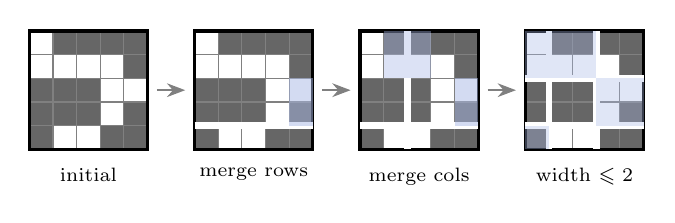
\begin{tikzpicture}[scale=0.30]
% Helper for drawing a 5x5 matrix
% State 1
\begin{scope}
\foreach \r/\d [count=\ri from 0] in {
0/{0,1,1,1,1},1/{0,0,0,0,1},2/{1,1,1,0,0},3/{1,1,1,0,1},4/{1,0,0,1,1}}{
\foreach \v [count=\ci from 0] in \d {
\ifnum\v=1 \fill[black!60] (\ci,4-\ri) rectangle ++(1,1);
\else \fill[white] (\ci,4-\ri) rectangle ++(1,1); \fi}}
\draw[step=1,gray] (0,0) grid (5,5);
\draw[very thick] (0,0) rectangle (5,5);
\node[below,font=\scriptsize] at (2.5,-0.4) {initial};
\end{scope}
\draw[-{Stealth},thick,gray] (5.4,2.5)--(6.6,2.5);
% State 2: merge rows 3,4
\begin{scope}[shift={(7,0)}]
\foreach \r/\d [count=\ri from 0] in {
0/{0,1,1,1,1},1/{0,0,0,0,1},2/{1,1,1,0,0},3/{1,1,1,0,1},4/{1,0,0,1,1}}{
\foreach \v [count=\ci from 0] in \d {
\ifnum\v=1 \fill[black!60] (\ci,4-\ri) rectangle ++(1,1);
\else \fill[white] (\ci,4-\ri) rectangle ++(1,1); \fi}}
\draw[step=1,gray] (0,0) grid (5,5);
\draw[very thick] (0,0) rectangle (5,5);
\draw[white,line width=2.5pt] (0,1)--(5,1);
\fill[nczone,opacity=0.5] (4,1) rectangle (5,3);
\node[below,font=\scriptsize] at (2.5,-0.4) {merge rows};
\end{scope}
\draw[-{Stealth},thick,gray] (12.4,2.5)--(13.6,2.5);
% State 3: also merge cols 2,3
\begin{scope}[shift={(14,0)}]
\foreach \r/\d [count=\ri from 0] in {
0/{0,1,1,1,1},1/{0,0,0,0,1},2/{1,1,1,0,0},3/{1,1,1,0,1},4/{1,0,0,1,1}}{
\foreach \v [count=\ci from 0] in \d {
\ifnum\v=1 \fill[black!60] (\ci,4-\ri) rectangle ++(1,1);
\else \fill[white] (\ci,4-\ri) rectangle ++(1,1); \fi}}
\draw[step=1,gray] (0,0) grid (5,5);
\draw[very thick] (0,0) rectangle (5,5);
\draw[white,line width=2.5pt] (0,1)--(5,1);
\draw[white,line width=2.5pt] (2,0)--(2,5);
\fill[nczone,opacity=0.5] (4,1) rectangle (5,3);
\fill[nczone,opacity=0.4] (1,3) rectangle (3,5);
\node[below,font=\scriptsize] at (2.5,-0.4) {merge cols};
\end{scope}
\draw[-{Stealth},thick,gray] (19.4,2.5)--(20.6,2.5);
% State 4: late
\begin{scope}[shift={(21,0)}]
\foreach \r/\d [count=\ri from 0] in {
0/{0,1,1,1,1},1/{0,0,0,0,1},2/{1,1,1,0,0},3/{1,1,1,0,1},4/{1,0,0,1,1}}{
\foreach \v [count=\ci from 0] in \d {
\ifnum\v=1 \fill[black!60] (\ci,4-\ri) rectangle ++(1,1);
\else \fill[white] (\ci,4-\ri) rectangle ++(1,1); \fi}}
\draw[step=1,gray] (0,0) grid (5,5);
\draw[very thick] (0,0) rectangle (5,5);
\draw[white,line width=2.5pt] (0,1)--(5,1);
\draw[white,line width=2.5pt] (0,3)--(5,3);
\draw[white,line width=2.5pt] (1,0)--(1,5);
\draw[white,line width=2.5pt] (3,0)--(3,5);
\fill[nczone,opacity=0.35] (0,3) rectangle (1,5);
\fill[nczone,opacity=0.35] (1,3) rectangle (3,5);
\fill[nczone,opacity=0.35] (3,1) rectangle (5,3);
\fill[nczone,opacity=0.35] (0,0) rectangle (1,1);
\node[below,font=\scriptsize] at (2.5,-0.4) {width $\leq 2$};
\end{scope}
\end{tikzpicture}
\end{frame}

%% ============== SLIDE 4: The gap ==============
\begin{frame}{The gap: static yes, dynamic no}
\begin{beamercolorbox}[wd=\textwidth,sep=0.55ex,rounded=true]{block body}
{\small Matrix viewpoint: a standard lens on twin-width; compact representations [PSZ] are the starting point here.}
\end{beamercolorbox}

\smallskip
\begin{columns}[T]
\begin{column}{0.46\textwidth}
\begin{block}{Static compact representation {\small[PSZ, STACS'22]}}
\begin{itemize}
\item $\Oh_d(n)$ bits of space
\item Queries in $\Oh_d(\log\log n)$
\item The matrix is initialized once
\end{itemize}
\end{block}
\end{column}
\begin{column}{0.46\textwidth}
\begin{alertblock}{Our dynamic question}
\begin{itemize}
\item Support \texttt{QueryBit} and \texttt{Update}
\item $M$ stays $d$-twin-ordered at every moment
\item Near-linear memory on word RAM
\end{itemize}
\end{alertblock}
\end{column}
\end{columns}

\bigskip
\centering
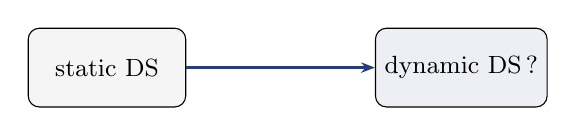
\begin{tikzpicture}
\node[draw,rounded corners,minimum width=2cm,minimum height=1cm,fill=gray!8] (s) at (0,0) {\small static DS};
\node[draw,rounded corners,minimum width=2cm,minimum height=1cm,fill=darkblue!8] (d) at (4.5,0) {\small dynamic DS\,?};
\draw[-{Stealth[length=5pt]},very thick,darkblue] (s)--(d);
\end{tikzpicture}

\smallskip
{\small Can compactness survive single-cell flips, without paying for a full rebuild every time?}
\end{frame}

%% ============== SLIDE 5: Main theorem ==============
\begin{frame}{Main theorem}
\begin{block}{\textbf{Theorem 1.}}
Let $d\in\mathbb{N}$ and $M\in\{0,1\}^{n\times n}$ be updated over time, always remaining $d$-twin-ordered.
There exists a dynamic data structure using $\Oh_d(n)$ memory supporting:
\begin{itemize}
\item $\mathtt{Init}(n,\mathcal{K})$ \hfill $\Oh_d\!\bigl((n+|\mathcal{K}|)\log\log n\bigr)$
\item $\mathtt{QueryBit}(i,j)$ \hfill $\Oh(\log\log n)$ expected worst-case
\item $\mathtt{Update}(i,j)$ \hfill $\Oh(\log\log n)$ expected worst-case
\end{itemize}
\end{block}

\vspace{-0.2em}
{\small $\mathcal{K}$: list of disjoint rectangles covering all ones. \quad Word RAM model: $\Oh_d(n)$ memory $=\Oh_d(n\log n)$ bits.}

\smallskip
{\small Only initialization time and memory depend on $d$.}

\medskip
\centering
\begin{tabular}{lccc}
\toprule
& \textbf{Space} & \textbf{Query} & \textbf{Update}\\
\midrule
Static [PSZ'22] & $\Oh_d(n)$ bits & $\Oh_d(\log\log n)$ & ---\\
\textbf{Dynamic [this work]} & $\Oh_d(n)$ memory & $\Oh(\log\log n)$ & $\Oh(\log\log n)$\\
\bottomrule
\end{tabular}
\end{frame}

%% ============== SLIDE 6: Slabs ==============
\begin{frame}{Slabs: why near-linear space is possible}
A \emph{slab} is a zone $M\bigl[[a,b],[c,d]\bigr]$ entirely filled with ones.

A \emph{slab decomposition} $\mathcal{K}$: pairwise disjoint slabs covering all ones.

\medskip
\begin{alertblock}{}
$|\mathcal{K}| \leq d(2n-2)+1$
\end{alertblock}

{\small Every $d$-twin-ordered matrix admits an $\Oh_d(n)$-size rectangle description of all ones.}

\bigskip
\begin{columns}[T]
\begin{column}{0.42\textwidth}
\centering
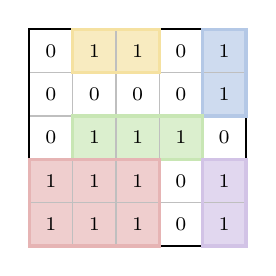
\begin{tikzpicture}[scale=0.55]
\fillslab{slab4}{1}{1}{2}{3}{5}
\fillslab{slab2}{1}{2}{5}{5}{5}
\fillslab{slab3}{3}{3}{2}{4}{5}
\fillslab{slab1}{4}{5}{1}{3}{5}
\fillslab{slab5}{4}{5}{5}{5}{5}
\foreach \r/\d [count=\ri from 0] in {
0/{0,1,1,0,1},
1/{0,0,0,0,1},
2/{0,1,1,1,0},
3/{1,1,1,0,1},
4/{1,1,1,0,1}}{
  \foreach \v [count=\ci from 0] in \d {
    \node[font=\scriptsize] at (\ci+0.5,4.5-\ri) {\v};
  }
}
\draw[step=1,gray!50] (0,0) grid (5,5);
\draw[thick] (0,0) rectangle (5,5);
\drawslab{slab4}{1}{1}{2}{3}{5}
\drawslab{slab2}{1}{2}{5}{5}{5}
\drawslab{slab3}{3}{3}{2}{4}{5}
\drawslab{slab1}{4}{5}{1}{3}{5}
\drawslab{slab5}{4}{5}{5}{5}{5}
\end{tikzpicture}
\end{column}
\begin{column}{0.54\textwidth}
{\small
\textbf{Example slab decomposition:}\\[4pt]
$\mathcal{K}=\{$\\
\hspace*{1em}$M\bigl[[1,1],[2,3]\bigr],\ M\bigl[[1,2],[5,5]\bigr],$\\
\hspace*{1em}$M\bigl[[3,3],[2,4]\bigr],$\\
\hspace*{1em}$M\bigl[[4,5],[1,3]\bigr],\ M\bigl[[4,5],[5,5]\bigr]$\\
$\}$\\[4pt]

\medskip
Each slab stored as four coordinates $(a,b,c,d)$.
}
\end{column}
\end{columns}
\end{frame}

%% ============== SLIDE 7: Canonical slabs ==============
\begin{frame}{Canonical slabs: normalization for rebuilding}
\vspace{-0.2em}
{\small
\begin{itemize}
\setlength\itemsep{0.15em}
\item An $i$-\emph{strip}: a width-$1$ all-ones slab $(a,b,i,i)$, maximal up/down in column $i$
\item $\strips_i$: the set of all $i$-strips
\item \emph{Siblings}: the same row interval $(a,b)$ persists as a strip through every column in between
\end{itemize}
}

\begin{beamercolorbox}[wd=\textwidth,sep=0.65ex,rounded=true]{block body alerted}
\footnotesize A \emph{canonical slab} is the union of one sibling class. The family of all of them is $\mathcal{R}$.
\end{beamercolorbox}

\vspace{-0.2em}
\[
|\mathcal{R}| \leq 4f_d(n+2)+4n
\]
{\footnotesize Canonicalization gives each rebuild a normalized slab family; every strip is assigned once, and size remains $\Oh_d(n)$.}

{\scriptsize Same matrix on both sides: the left decomposition is valid, but it merges different sibling classes.}

\smallskip
\begin{columns}[T,onlytextwidth]
\begin{column}{0.48\textwidth}
\centering
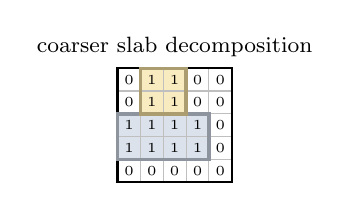
\begin{tikzpicture}[scale=0.29]
\node[above,font=\footnotesize] at (2.5,5.08) {coarser slab decomposition};
\fillslab{coarsefill}{3}{4}{1}{4}{5}
\fillslab{slab4}{1}{2}{2}{3}{5}
\foreach \r/\d [count=\ri from 0] in {
0/{0,1,1,0,0},
1/{0,1,1,0,0},
2/{1,1,1,1,0},
3/{1,1,1,1,0},
4/{0,0,0,0,0}}{
  \foreach \v [count=\ci from 0] in \d {
    \node[font=\tiny] at (\ci+0.5,4.5-\ri) {\v};
  }
}
\draw[step=1,gray!50] (0,0) grid (5,5);
\draw[thick] (0,0) rectangle (5,5);
\draw[coarsefill!70!black,very thick] (0,1) rectangle (4,3);
\draw[slab4!70!black,very thick] (1,3) rectangle (3,5);
\end{tikzpicture}
\end{column}
\begin{column}{0.48\textwidth}
\centering
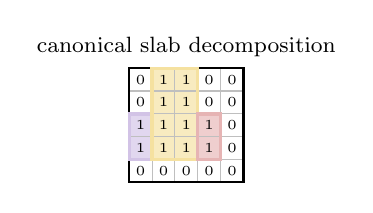
\begin{tikzpicture}[scale=0.29]
\node[above,font=\footnotesize] at (2.5,5.08) {canonical slab decomposition};
\fillslab{slab5}{3}{4}{1}{1}{5}
\fillslab{slab4}{1}{4}{2}{3}{5}
\fillslab{slab1}{3}{4}{4}{4}{5}
\foreach \r/\d [count=\ri from 0] in {
0/{0,1,1,0,0},
1/{0,1,1,0,0},
2/{1,1,1,1,0},
3/{1,1,1,1,0},
4/{0,0,0,0,0}}{
  \foreach \v [count=\ci from 0] in \d {
    \node[font=\tiny] at (\ci+0.5,4.5-\ri) {\v};
  }
}
\draw[step=1,gray!50] (0,0) grid (5,5);
\draw[thick] (0,0) rectangle (5,5);
\drawslab{slab5}{3}{4}{1}{1}{5}
\drawslab{slab4}{1}{4}{2}{3}{5}
\drawslab{slab1}{3}{4}{4}{4}{5}
\end{tikzpicture}
\end{column}
\end{columns}
\end{frame}

%% ============== SLIDE 8: Running example part I ==============
\begin{frame}{Running example I: sweep detects disappearing strips}
\begin{columns}[T,onlytextwidth]
\begin{column}{0.32\textwidth}
\vspace{-0.2cm}
{\footnotesize\textbf{One left-to-right round}}
\[
\resizebox{\linewidth}{!}{$
\begin{aligned}
O_i &\coloneqq \{[a,b]\mid (a,b,i,d')\in\mathcal{K},\ d'\!\geq\! i\},\\
C_i &\coloneqq \{[a,b]\mid (a,b,c',i)\in\mathcal{K},\ c'\!\leq\! i\},\\
B_i &\coloneqq \strips_i \setminus \strips_{i+1}.
\end{aligned}
$}
\]

\begin{beamercolorbox}[wd=\linewidth,sep=0.65ex,rounded=true]{block body alerted}
\footnotesize Invariant: before round $i$, $\mathbb{S}$ stores exactly $\strips_i$.
\end{beamercolorbox}

\smallskip
{\scriptsize
\begin{itemize}
\setlength\itemsep{0.18em}
\item $C_i$ closes slabs ending at column $i$
\item $O_{i+1}$ opens slabs starting at column $i+1$
\item Re-test only touched intervals; failed tests form $B_i$
\end{itemize}
}

\smallskip
{\scriptsize First half of $\mathtt{Decompose}$: record where canonical slabs end.}
\end{column}
\begin{column}{0.66\textwidth}
\centering
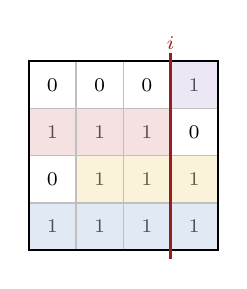
\begin{tikzpicture}[scale=0.60]
\foreach \r/\d [count=\ri from 0] in {
0/{0,0,0,1},1/{1,1,1,0},2/{0,1,1,1},3/{1,1,1,1}}{
\foreach \v [count=\ci from 0] in \d {
\node[font=\scriptsize] at (\ci+0.5,3.5-\ri) {\v};
}}
% Color the slabs: K = {(2,2,1,3),(3,3,2,4),(4,4,1,4),(1,1,4,4)}
\fill[slab1,opacity=0.4] (0,2) rectangle (3,3); % (2,2,1,3)
\fill[slab4,opacity=0.4] (1,1) rectangle (4,2); % (3,3,2,4)
\fill[slab2,opacity=0.4] (0,0) rectangle (4,1); % (4,4,1,4)
\fill[slab5,opacity=0.4] (3,3) rectangle (4,4); % (1,1,4,4)
\draw[step=1,gray!50] (0,0) grid (4,4);
\draw[thick] (0,0) rectangle (4,4);
\draw[darkred,very thick] (3,-0.18) -- (3,4.18);
\node[darkred,font=\scriptsize] at (3,4.38) {$i$};
\end{tikzpicture}

\smallskip
{\scriptsize
\renewcommand{\arraystretch}{1.28}
\resizebox{\linewidth}{!}{%
\begin{tabular}{@{}c|c|c|>{\columncolor{softred}}c@{}}
 & before: $\strips_i$ & after: $\strips_{i+1}$ & \textbf{disappears: $B_i$}\\
\hline
\rowcolor{slab4!18}
$i\!=\!1$ & $\{[2,2],[4,4]\}$ & $\{[2,4]\}$ & \textbf{$\{[2,2],[4,4]\}$}\\
\hline
$i\!=\!2$ & $\{[2,4]\}$ & $\{[2,4]\}$ & \textbf{$\varnothing$}\\
\hline
\rowcolor{slab1!12}
$i\!=\!3$ & $\{[2,4]\}$ & $\{[1,1],[3,4]\}$ & \textbf{$\{[2,4]\}$}\\
\hline
$i\!=\!4$ & $\{[1,1],[3,4]\}$ & $\varnothing$ & \textbf{$\{[1,1],[3,4]\}$}\\
\end{tabular}
}
}

\vspace{0.25em}
{\scriptsize\color{gray!75!black}Read the red column as ``the strips whose canonical slabs end here''.}
\end{column}
\end{columns}
\end{frame}

%% ============== SLIDE 9: Running example part II ==============
\begin{frame}{Running example II: starts and ends form canonical slabs}
\begin{columns}[T,onlytextwidth]
\begin{column}{0.30\textwidth}
{\scriptsize A symmetric right-to-left sweep gives}
\[
A_i \coloneqq \strips_i \setminus \strips_{i-1}
\]

\vspace{-0.4em}
\scriptsize
\begin{itemize}
\setlength\itemsep{0.18em}
\item $A_i$ opens a sibling class
\item $B_i$ closes the same row interval later
\item $\mathsf{slab\_start}[a]$ stores its opening column
\end{itemize}

\begin{beamercolorbox}[wd=\linewidth,sep=0.65ex,rounded=true]{block body alerted}
\footnotesize On closing $[a,b]\in B_i$, output $(a,b,\mathsf{slab\_start}[a],i)$.
\end{beamercolorbox}

\smallskip
{\scriptsize $\mathtt{Decompose}(n,\mathcal{K})$ computes $\mathcal{R}$ in $\Oh(n+|\mathcal{K}|\log\log n)$.}
\end{column}
\begin{column}{0.68\textwidth}
\centering
{\scriptsize
\renewcommand{\arraystretch}{1.32}
\resizebox{\linewidth}{!}{%
\begin{tabular}{@{}c|c|c|>{\columncolor{softgreen}}c@{}}
 & opens: $A_i$ & closes: $B_i$ & \textbf{canonical slabs output in round $i$}\\
\hline
\rowcolor{slab4!18}
$i\!=\!1$ & $\{[2,2],[4,4]\}$ & $\{[2,2],[4,4]\}$ & \textbf{$(2,2,1,1),\ (4,4,1,1)$}\\
\hline
$i\!=\!2$ & $\{[2,4]\}$ & $\varnothing$ & --\\
\hline
\rowcolor{slab1!12}
$i\!=\!3$ & $\varnothing$ & $\{[2,4]\}$ & \textbf{$(2,4,2,3)$}\\
\hline
$i\!=\!4$ & $\{[1,1],[3,4]\}$ & $\{[1,1],[3,4]\}$ & \textbf{$(1,1,4,4),\ (3,4,4,4)$}\\
\end{tabular}
}
}

\vspace{0.35em}
{\scriptsize\color{gray!75!black}Example: at $i=3$, the interval $[2,4]$ closes and $\mathsf{slab\_start}[2]=2$, hence $(2,4,2,3)$.}

\vspace{0.25em}
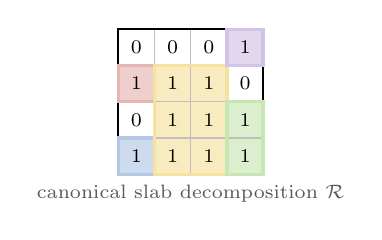
\begin{tikzpicture}[scale=0.46]
\fillslab{slab1}{2}{2}{1}{1}{4}
\fillslab{slab2}{4}{4}{1}{1}{4}
\fillslab{slab4}{2}{4}{2}{3}{4}
\fillslab{slab5}{1}{1}{4}{4}{4}
\fillslab{slab3}{3}{4}{4}{4}{4}
\foreach \r/\d [count=\ri from 0] in {
0/{0,0,0,1},
1/{1,1,1,0},
2/{0,1,1,1},
3/{1,1,1,1}}{
  \foreach \v [count=\ci from 0] in \d {
    \node[font=\scriptsize] at (\ci+0.5,3.5-\ri) {\v};
  }
}
\draw[step=1,gray!50] (0,0) grid (4,4);
\draw[thick] (0,0) rectangle (4,4);
\drawslab{slab1}{2}{2}{1}{1}{4}
\drawslab{slab2}{4}{4}{1}{1}{4}
\drawslab{slab4}{2}{4}{2}{3}{4}
\drawslab{slab5}{1}{1}{4}{4}{4}
\drawslab{slab3}{3}{4}{4}{4}{4}
\node[font=\scriptsize,gray!70!black] at (2,-0.55) {canonical slab decomposition $\mathcal{R}$};
\end{tikzpicture}
\end{column}
\end{columns}
\end{frame}

%% ============== SLIDE 10: Amortized structure ==============
\begin{frame}{Amortized structure: $\mathbb{P}$ for slabs, $\mathbb{Q}$ for recent flips}

{\footnotesize Keep the last canonical slab family $\mathcal{P}$ inside a static point-location structure $\mathbb{P}$. New flips are buffered in $\mathbb{Q}$ instead of merged immediately.}

\smallskip
\begin{columns}[T,onlytextwidth]
\begin{column}{0.43\textwidth}
\centering
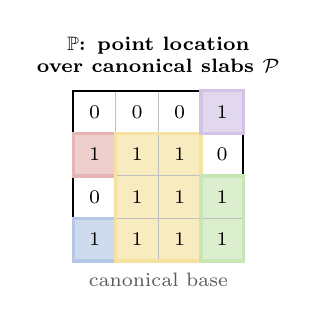
\begin{tikzpicture}[scale=0.54]
\node[font=\scriptsize\bfseries,align=center] at (2,4.85) {$\mathbb{P}$: point location\\over canonical slabs $\mathcal{P}$};
\fillslab{slab1}{2}{2}{1}{1}{4}
\fillslab{slab2}{4}{4}{1}{1}{4}
\fillslab{slab4}{2}{4}{2}{3}{4}
\fillslab{slab5}{1}{1}{4}{4}{4}
\fillslab{slab3}{3}{4}{4}{4}{4}
\foreach \r/\d [count=\ri from 0] in {
0/{0,0,0,1},
1/{1,1,1,0},
2/{0,1,1,1},
3/{1,1,1,1}}{
  \foreach \v [count=\ci from 0] in \d {
    \node[font=\scriptsize] at (\ci+0.5,3.5-\ri) {\v};
  }
}
\draw[step=1,gray!50] (0,0) grid (4,4);
\draw[thick] (0,0) rectangle (4,4);
\drawslab{slab1}{2}{2}{1}{1}{4}
\drawslab{slab2}{4}{4}{1}{1}{4}
\drawslab{slab4}{2}{4}{2}{3}{4}
\drawslab{slab5}{1}{1}{4}{4}{4}
\drawslab{slab3}{3}{4}{4}{4}{4}
\node[font=\scriptsize,align=center,gray!70!black] at (2,-0.45) {canonical base};
\end{tikzpicture}

\end{column}
\begin{column}{0.55\textwidth}
\centering
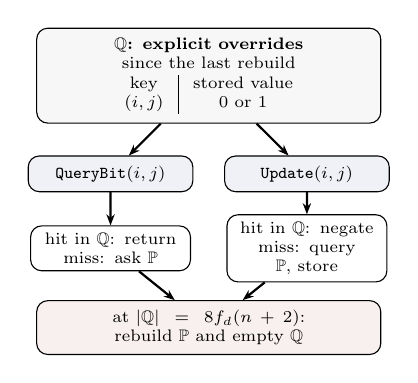
\begin{tikzpicture}[scale=0.86,transform shape,font=\scriptsize,
  box/.style={draw,rounded corners,align=center,fill=gray!6,inner sep=4pt},
  op/.style={draw,rounded corners,align=center,fill=darkblue!7,inner sep=4pt,text width=2.15cm},
  smallbox/.style={draw,rounded corners,align=center,fill=white,inner sep=3pt,text width=2.15cm}]
\node[box,text width=4.8cm] (q) at (0,0) {\textbf{$\mathbb{Q}$: explicit overrides}\\since the last rebuild\\[2pt]
\begin{tabular}{c|c}
key & stored value\\
$(i,j)$ & $0$ or $1$
\end{tabular}};
\node[op] (query) at (-1.45,-1.45) {$\mathtt{QueryBit}(i,j)$};
\node[op] (update) at (1.45,-1.45) {$\mathtt{Update}(i,j)$};
\node[smallbox] (qhit) at (-1.45,-2.55) {hit in $\mathbb{Q}$: return\\miss: ask $\mathbb{P}$};
\node[smallbox] (store) at (1.45,-2.55) {hit in $\mathbb{Q}$: negate\\miss: query $\mathbb{P}$, store};
\node[box,fill=darkred!7,text width=4.8cm] (threshold) at (0,-3.72)
  {at $|\mathbb{Q}|=8f_d(n+2)$: rebuild $\mathbb{P}$ and empty $\mathbb{Q}$};
\draw[-{Stealth[length=4pt]},thick] (q)--(query);
\draw[-{Stealth[length=4pt]},thick] (q)--(update);
\draw[-{Stealth[length=4pt]},thick] (query)--(qhit);
\draw[-{Stealth[length=4pt]},thick] (update)--(store);
\draw[-{Stealth[length=4pt]},thick] (qhit)--(threshold);
\draw[-{Stealth[length=4pt]},thick] (store)--(threshold);
\end{tikzpicture}
\end{column}
\end{columns}

\smallskip
{\footnotesize \textbf{Invariant:} $(i,j)\in\mathbb{Q} \Rightarrow M[i,j]=\mathbb{Q}[i,j]$. \;
$(i,j)\notin\mathbb{Q} \Rightarrow M[i,j]=1 \iff (i,j)$ lies in a base slab of $\mathbb{P}$.}

\end{frame}

%% ============== SLIDE 11: Rebuilding ==============
\begin{frame}{Rebuilding $\mathbb{P}$: create a fresh decomposition}

{\footnotesize Rebuilding starts from two extracted lists: old slabs $\mathcal{P}$ from $\mathbb{P}$, and buffered values $\mathcal{Q}$ from $\mathbb{Q}$.}

\vspace{-0.15em}
\centering
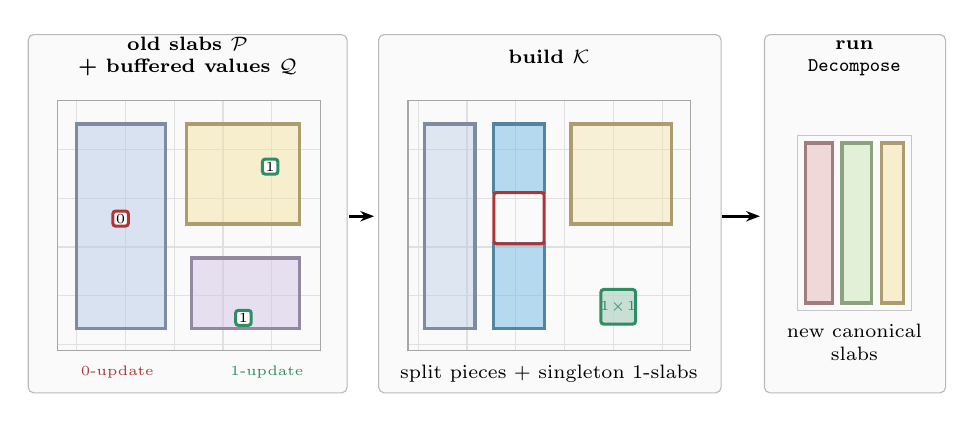
\begin{tikzpicture}[x=1cm,y=1cm,font=\scriptsize,
  panelbox/.style={draw=gray!55,rounded corners=2pt,fill=gray!4},
  paneltitle/.style={font=\scriptsize\bfseries,align=center},
  updzero/.style={draw=updatezero,line width=1.1pt,fill=white,rounded corners=1pt,inner sep=1.1pt,font=\tiny\bfseries},
  updone/.style={draw=updateone,line width=1.1pt,fill=white,rounded corners=1pt,inner sep=1.1pt,font=\tiny\bfseries},
  note/.style={font=\scriptsize,align=center}]

\node[panelbox,minimum width=4.05cm,minimum height=4.55cm,anchor=south west] (oldbox) at (0,0) {};
\node[paneltitle] at (2.03,4.28) {old slabs $\mathcal{P}$\\+ buffered values $\mathcal{Q}$};
\draw[step=0.62,gray!24] (0.38,0.55) grid (3.72,3.72);
\draw[gray!70] (0.38,0.55) rectangle (3.72,3.72);
\fill[slab2,opacity=0.48] (0.62,0.82) rectangle (1.75,3.42);
\fill[slab4,opacity=0.48] (2.02,2.15) rectangle (3.45,3.42);
\fill[slab5,opacity=0.48] (2.08,0.82) rectangle (3.45,1.72);
\draw[slab2!70!black,very thick] (0.62,0.82) rectangle (1.75,3.42);
\draw[slab4!70!black,very thick] (2.02,2.15) rectangle (3.45,3.42);
\draw[slab5!70!black,very thick] (2.08,0.82) rectangle (3.45,1.72);
\node[updzero] at (1.18,2.22) {$0$};
\node[updone] at (2.74,0.96) {$1$};
\node[updone] at (3.08,2.88) {$1$};
\node[updatezero,anchor=west,font=\tiny] at (0.55,0.27) {$0$-update};
\node[updateone,anchor=west,font=\tiny] at (2.45,0.27) {$1$-update};

\node[panelbox,minimum width=4.35cm,minimum height=4.55cm,anchor=south west] (kbox) at (4.45,0) {};
\node[paneltitle] at (6.62,4.28) {build $\mathcal{K}$};
\draw[step=0.62,gray!24] (4.83,0.55) grid (8.42,3.72);
\draw[gray!70] (4.83,0.55) rectangle (8.42,3.72);
\fill[slab2,opacity=0.40] (5.04,0.82) rectangle (5.68,3.42);
\fill[splitpiece,opacity=0.52] (5.92,0.82) rectangle (6.56,1.90);
\fill[splitpiece,opacity=0.52] (5.92,2.55) rectangle (6.56,3.42);
\fill[slab4,opacity=0.40] (6.90,2.15) rectangle (8.18,3.42);
\fill[updateone!35,opacity=0.75] (7.28,0.88) rectangle (7.72,1.32);
\draw[slab2!70!black,very thick] (5.04,0.82) rectangle (5.68,3.42);
\draw[splitpiece!70!black,very thick] (5.92,0.82) rectangle (6.56,1.90);
\draw[splitpiece!70!black,very thick] (5.92,2.55) rectangle (6.56,3.42);
\draw[updatezero,line width=1.1pt,rounded corners=1pt] (5.92,1.90) rectangle (6.56,2.55);
\draw[slab4!70!black,very thick] (6.90,2.15) rectangle (8.18,3.42);
\draw[updateone,line width=1.1pt,rounded corners=1pt] (7.28,0.88) rectangle (7.72,1.32);
\node[font=\tiny\bfseries,updateone] at (7.50,1.10) {$1\!\times\!1$};
\node[note] at (6.62,0.25) {split pieces + singleton $1$-slabs};

\node[panelbox,minimum width=2.30cm,minimum height=4.55cm,anchor=south west] (decompbox) at (9.35,0) {};
\node[paneltitle] at (10.50,4.25) {run\\$\mathtt{Decompose}$};
\draw[gray!45] (9.78,1.05) rectangle (11.22,3.28);
\fill[slab1,opacity=0.48] (9.88,1.15) rectangle (10.22,3.18);
\fill[slab3,opacity=0.48] (10.34,1.15) rectangle (10.72,3.18);
\fill[slab4,opacity=0.48] (10.84,1.15) rectangle (11.12,3.18);
\draw[slab1!70!black,very thick] (9.88,1.15) rectangle (10.22,3.18);
\draw[slab3!70!black,very thick] (10.34,1.15) rectangle (10.72,3.18);
\draw[slab4!70!black,very thick] (10.84,1.15) rectangle (11.12,3.18);
\node[note] at (10.50,0.65) {new canonical\\slabs};

\draw[-{Stealth[length=5pt]},very thick] (4.08,2.25)--(4.40,2.25);
\draw[-{Stealth[length=5pt]},very thick] (8.82,2.25)--(9.30,2.25);
\end{tikzpicture}

\vspace{-0.35em}
\begin{beamercolorbox}[wd=0.92\textwidth,sep=0.7ex,rounded=true,center]{block body alerted}
\scriptsize Split old slabs at buffered $0$-updates; add uncovered $1$-updates as $1\!\times\!1$ slabs. \quad
$|\mathcal{K}| \leq |\mathcal{P}| + 2|\mathcal{Q}|$.
\end{beamercolorbox}
\end{frame}

%% ============== SLIDE 12: De-amortization ==============
\begin{frame}{Worst-case updates: epochs and snapshot copies}

{\footnotesize Let $L=8f_d(n+2)$ and split the update sequence into epochs of length $L$. A rebuild that costs $\Oh(L\log\log n)$ is paid for gradually.}

\smallskip
\begin{beamercolorbox}[wd=\textwidth,sep=0.65ex,rounded=true]{block body}
\scriptsize Active copy answers online operations. Frozen snapshot is read-only, so the next copy can be initialized while the active one keeps changing.
\end{beamercolorbox}

\smallskip
\centering
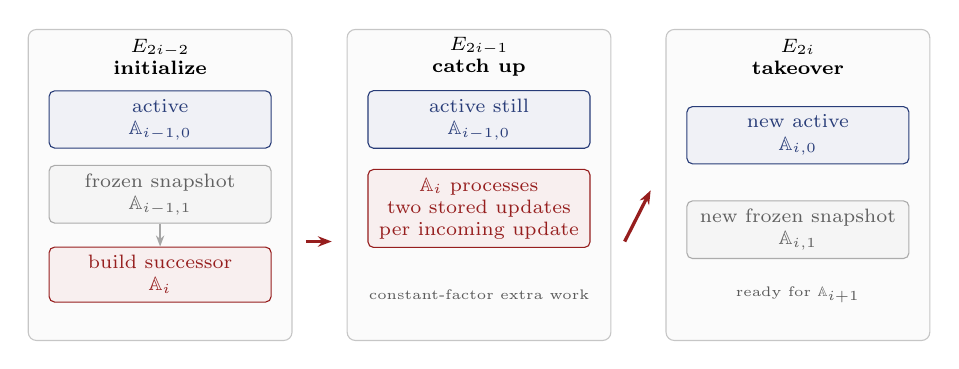
\begin{tikzpicture}[x=1cm,y=1cm,font=\scriptsize,
  phase/.style={draw=gray!45,rounded corners=3pt,fill=gray!3,minimum width=3.35cm,minimum height=3.95cm,anchor=north},
  title/.style={font=\scriptsize\bfseries,align=center},
  copy/.style={draw,rounded corners=2pt,align=center,inner sep=3pt,minimum width=2.82cm},
  active/.style={copy,draw=darkblue,text=darkblue,fill=darkblue!7},
  frozen/.style={copy,draw=gray!65,text=gray!75!black,fill=gray!8},
  next/.style={copy,draw=darkred,text=darkred,fill=darkred!7}]

\node[phase] (p1) at (0,0) {};
\node[phase] (p2) at (4.05,0) {};
\node[phase] (p3) at (8.10,0) {};

\node[title] at (0,-0.35) {$E_{2i-2}$\\initialize};
\node[active] (a10) at (0,-1.15) {active\\$\mathbb{A}_{i-1,0}$};
\node[frozen] (f10) at (0,-2.10) {frozen snapshot\\$\mathbb{A}_{i-1,1}$};
\node[next] (n10) at (0,-3.12) {build successor\\$\mathbb{A}_i$};
\draw[-{Stealth[length=4pt]},gray!70,thick] (f10)--(n10);

\node[title] at (4.05,-0.35) {$E_{2i-1}$\\catch up};
\node[active] at (4.05,-1.15) {active still\\$\mathbb{A}_{i-1,0}$};
\node[next] at (4.05,-2.28) {$\mathbb{A}_i$ processes\\two stored updates\\per incoming update};
\node[font=\tiny,gray!70!black,align=center] at (4.05,-3.38) {constant-factor extra work};

\node[title] at (8.10,-0.35) {$E_{2i}$\\takeover};
\node[active] at (8.10,-1.35) {new active\\$\mathbb{A}_{i,0}$};
\node[frozen] at (8.10,-2.55) {new frozen snapshot\\$\mathbb{A}_{i,1}$};
\node[font=\tiny,gray!70!black,align=center] at (8.10,-3.38) {ready for $\mathbb{A}_{i+1}$};

\draw[-{Stealth[length=5pt]},very thick,darkred] (1.85,-2.70)--(2.18,-2.70);
\draw[-{Stealth[length=5pt]},very thick,darkred] (5.90,-2.70)--(6.23,-2.05);
\end{tikzpicture}

\smallskip
{\footnotesize This turns the amortized rebuild threshold into $\Oh(\log\log n)$ expected worst-case update time.}
\end{frame}

%% ============== SLIDE 13: Take-away ==============
\begin{frame}{Take-away}

\begin{alertblock}{}
For every fixed $d$, a dynamically updated $d$-twin-ordered matrix admits:\\[2pt]
\[
\Oh_d(n)\ \text{memory},\qquad
\Oh(\log\log n)\ \text{expected worst-case query and update time.}
\]
\end{alertblock}

\medskip
\centering
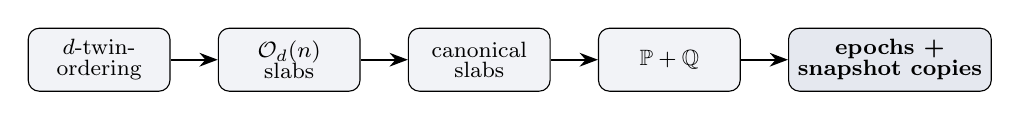
\begin{tikzpicture}[node distance=0.6cm,font=\small,
  box/.style={draw,rounded corners,minimum height=0.8cm,minimum width=1.8cm,fill=darkblue!6,align=center,font=\footnotesize}]
\node[box] (tw) {$d$-twin-\\[-2pt]ordering};
\node[box,right=of tw] (sl) {$\Oh_d(n)$\\[-2pt]slabs};
\node[box,right=of sl] (cs) {canonical\\[-2pt]slabs};
\node[box,right=of cs] (pq) {$\mathbb{P}+\mathbb{Q}$};
\node[box,right=of pq,fill=darkblue!12,font=\footnotesize\bfseries,minimum width=2.25cm] (ds) {epochs +\\[-2pt]snapshot copies};
\draw[-{Stealth},thick] (tw)--(sl);
\draw[-{Stealth},thick] (sl)--(cs);
\draw[-{Stealth},thick] (cs)--(pq);
\draw[-{Stealth},thick] (pq)--(ds);
\end{tikzpicture}

\medskip
\begin{beamercolorbox}[wd=0.88\textwidth,sep=0.85ex,rounded=true,center]{block body}
{\small Canonical slabs make every rebuild small and well defined; $\mathbb{P}+\mathbb{Q}$ isolates recent flips; snapshot copies remove the amortization.}
\end{beamercolorbox}

\vspace{0.55cm}
\centering
{\Large\color{darkblue} Questions?}
\end{frame}

%% ============== BACKUP SLIDES ==============

\appendix

%% ============== BACKUP 14: Adhesive segment set ==============
\begin{frame}{Backup: adhesive segment set}

{\small A data structure $\mathbb{S}$ maintaining a dynamic set of pairwise disjoint, non-adjacent segments in $\{1,\ldots,n\}$.}

\medskip
Operations:
\begin{itemize}
\item $\mathtt{Containing}([a,b])$: return the segment of $S$ containing $[a,b]$
\item $\mathtt{Adjacent}([a,b])$: return segments adjacent to $[a,b]$
\item $\mathtt{Disjoint}([a,b])$: test disjointness from all segments
\item $\mathtt{Merge}([a,b])$: add $[a,b]$ and merge with adjacent segments
\item $\mathtt{Split}([a,b])$: remove $[a,b]$ from its containing segment
\end{itemize}

\medskip
{\small All operations in $\Oh(\log\log n)$ worst-case time. \quad $\Oh(n)$ memory. \quad Initialization in $\Oh(n)$.}

\bigskip
\centering
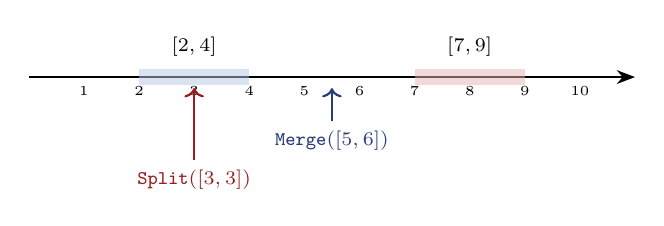
\begin{tikzpicture}[scale=0.7,font=\small]
\draw[thick,-{Stealth}] (0,0)--(11,0);
\foreach \x in {1,...,10} \node[below,font=\tiny] at (\x,0) {\x};
% Segments
\fill[slab2,opacity=0.5] (2,-0.15) rectangle (4,0.15);
\fill[slab1,opacity=0.5] (7,-0.15) rectangle (9,0.15);
\node[above,font=\scriptsize] at (3,0.2) {$[2,4]$};
\node[above,font=\scriptsize] at (8,0.2) {$[7,9]$};
% Merge example
\draw[->,thick,darkblue] (5.5,-0.8)--(5.5,-0.2);
\node[below,font=\scriptsize,darkblue] at (5.5,-0.8) {$\mathtt{Merge}([5,6])$};
% Split example
\draw[->,thick,darkred] (3,-1.5)--(3,-0.2);
\node[below,font=\scriptsize,darkred] at (3,-1.5) {$\mathtt{Split}([3,3])$};
\end{tikzpicture}
\end{frame}

%% ============== BACKUP 15: Why O_d(n) canonical slabs? ==============
\begin{frame}{Backup: why are there only $\Oh_d(n)$ canonical slabs?}

\begin{itemize}
\setlength\itemsep{0.05em}
\item A \emph{corner}: a $2\times 2$ zone whose two rows differ and two columns differ
\item \textbf{Lemma~1}: a $d$-twin-ordered matrix has $\leq f_d(n+2)$ corners, where $f_d = \tfrac{16}{3}(2d+3)^2\cdot 2^{4(2d+2)}$
\item Every ``internal'' canonical slab must intersect a corner
\item Boundary cases contribute only $4n$
\end{itemize}

\[
|\mathcal{R}| \leq 4f_d(n+2)+4n
\]

\vspace{-0.25em}
\centering
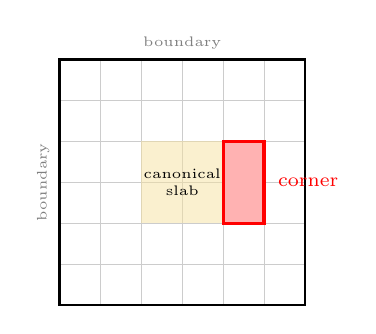
\begin{tikzpicture}[scale=0.52,font=\small]
% Matrix sketch
\draw[step=1,gray!40] (0,0) grid (6,6);
\draw[thick] (0,0) rectangle (6,6);
% A canonical slab
\fill[slab4,opacity=0.5] (2,2) rectangle (4,4);
\node[font=\tiny,align=center] at (3,3) {canonical\\slab};
% Corner witness
\fill[red!30] (4,3) rectangle (5,4);
\fill[red!30] (4,2) rectangle (5,3);
\draw[red,very thick] (4,2) rectangle (5,4);
\node[red,font=\scriptsize,right] at (5.1,3) {corner};
% Boundary labels
\node[gray,font=\tiny,rotate=90] at (-0.4,3) {boundary};
\node[gray,font=\tiny] at (3,6.4) {boundary};
\end{tikzpicture}
\end{frame}

%% ============== BACKUP 16: Rebuilding K in detail ==============
\begin{frame}{Backup: rebuilding $\mathcal{K}$ from $\mathcal{P}$ and $\mathcal{Q}$ in detail}

{\small Steps:}
\begin{enumerate}
\item Sort $\mathcal{Q}$ lexicographically in $\Oh(|\mathcal{Q}|)$ time
\item Assign 0-updates to slabs of $\mathcal{P}$ that contain them
\item For each affected slab $P=(a,b,c,d)$, process row batches $L_i$ of 0-updates with the same first coordinate
\item For each non-empty batch $L_i$: add $P[{<}i]$, split single-row slab $P[i]$ at sorted second coordinates from $L_i$, continue with $P[{>}i]$
\item Add $1\times 1$ slabs for uncovered 1-updates
\item Obtain $|\mathcal{K}|\leq |\mathcal{P}|+2|\mathcal{Q}|$, then run $\mathtt{Decompose}(n,\mathcal{K})$
\end{enumerate}

\smallskip
{\small Amortized over $8f_d(n+2)$ updates: $\Oh(\log\log n)$ per update.}

\bigskip
\centering
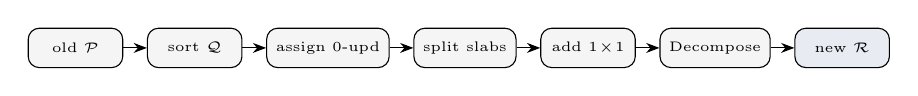
\begin{tikzpicture}[node distance=0.3cm,font=\tiny,
  box/.style={draw,rounded corners,minimum height=0.5cm,minimum width=1.2cm,fill=gray!8}]
\node[box] (p) {old $\mathcal{P}$};
\node[box,right=of p] (s) {sort $\mathcal{Q}$};
\node[box,right=of s] (a) {assign 0-upd};
\node[box,right=of a] (sp) {split slabs};
\node[box,right=of sp] (ad) {add $1\!\times\!1$};
\node[box,right=of ad] (dc) {Decompose};
\node[box,right=of dc,fill=darkblue!10] (nc) {new $\mathcal{R}$};
\draw[-{Stealth}] (p)--(s);
\draw[-{Stealth}] (s)--(a);
\draw[-{Stealth}] (a)--(sp);
\draw[-{Stealth}] (sp)--(ad);
\draw[-{Stealth}] (ad)--(dc);
\draw[-{Stealth}] (dc)--(nc);
\end{tikzpicture}

\medskip
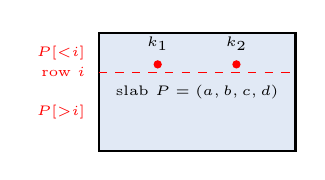
\begin{tikzpicture}[scale=0.5,font=\tiny]
% One slab being split
\fill[slab2!40] (0,0) rectangle (5,3);
\draw[thick] (0,0) rectangle (5,3);
\node at (2.5,1.5) {slab $P=(a,b,c,d)$};
% Row i
\draw[dashed,red] (0,2)--(5,2);
\node[left,red] at (-0.1,2.5) {$P[{<}i]$};
\node[left,red] at (-0.1,2) {row $i$};
\node[left,red] at (-0.1,1) {$P[{>}i]$};
% Split points in row i
\fill[red] (1.5,2.2) circle (3pt);
\fill[red] (3.5,2.2) circle (3pt);
\node[above] at (1.5,2.3) {$k_1$};
\node[above] at (3.5,2.3) {$k_2$};
\end{tikzpicture}
\end{frame}

\end{document}
